\documentclass[../../main.tex]{subfiles}
\begin{document}

{\bf [解]}

$g(x) = 0 \iff x = \pm 1, -4$ であり，この時題意の等式
\begin{align}
  f(x) - k g(x) = 0 \label{eq:1}
\end{align}
は成立しないので，
\begin{align}
  x \neq \pm 1, -4 \label{eq:2}
\end{align}
で考えれば良い．このときは$g(x) \neq 0$だから\cref{eq:1}の両辺を$g(x)$で割って
\begin{align}
  k
  &= \dfrac{f(x)}{g(x)} = \dfrac{x^2(x+8)}{(x^2-1)(x+4)} \\
  &= 1 + \dfrac{4x^2+x+4}{(x^2-1)(x+4)} \equiv h(x) \label{eq:3}
\end{align}
の相異なる実根の個数を考えれば良い．
これは $xy$ 平面での二つの曲線 $y=k$ と $y=h(x)$ の交点の数と等しい．
そこで$h(x)$の挙動を調べよう．一階微分は
\begin{align}
  h'(x)
  &= \dfrac{(8x+1)(x^2-1)(x+4) - (3x^2+8x-1)(4x^2+x+4)}{(x^2-1)^2 (x+4)^2} \\
  &= \dfrac{-4x^4 - 2x^3 - 20x^2 - 64x}{(x^2-1)^2 (x+4)^2} \\
  &= \dfrac{-2x(x+2)(2x^2 - 3x + 16)}{(x^2-1)^2 (x+4)^2}
\end{align}
である．ここで分子の第三因子について
\begin{align}
  2x^2 - 3x + 16 = 2\left(x - \dfrac{3}{4}\right)^2 + \dfrac{119}{8} > 0
\end{align}
だから増減表は以下のようになる．

\begin{table}[htb]
  \centering
  \caption{$h(x)$ の増減表}
  \begin{tabular}{c|c|c|c|c|c|c|c|c|c|c|c}
    $x$ & $\dots$ & $-4$ & $\dots$ & $-2$ & $\dots$ & $-1$ & $\dots$ & $0$ & $\dots$ & $1$ & $\dots$ \\ \hline
    $h'$ & $-$ & $\times$ & $-$ & $0$ & $+$ & $\times$ & $+$ & $0$ & $-$ & $\times$ & $-$ \\ \hline
    $h$ & $\searrow$ & $\times$ & $\searrow$ & $4$ & $\nearrow$ & $\times$ & $\nearrow$ & $0$ & $\searrow$ & $\times$ & $\searrow$
  \end{tabular}
\end{table}

また，極限値として以下をうる．
\begin{align}
  h(x) &\to +\infty \quad (x \to -4+0, -1-0, 1+0) \\
  h(x) &\to -\infty \quad (x \to -4-0, -1+0, 1-0) \\
  h(x) &\to 1 \quad (x \to \pm\infty)
\end{align}
したがって $y=h(x)$ のグラフは下図のようになる．

\begin{figure}[htb]
  \centering
  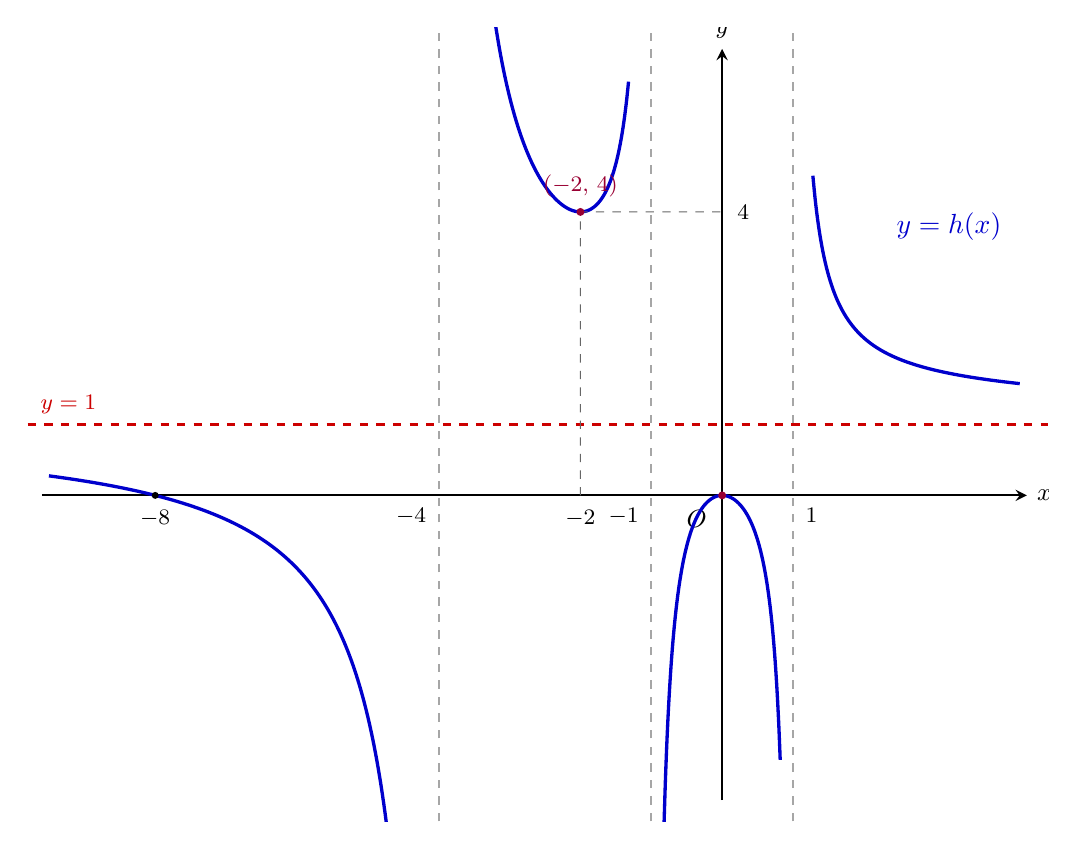
\begin{tikzpicture}[scale=0.9, >=stealth, every node/.style={font=\small}]

    % --- 1. クリッピング領域の設定 (描画範囲の外れを防ぐ) ---
    \clip (-9.8, -4.6) rectangle (4.6, 6.6);

    % --- 2. 漸近線 (Asymptotes) ---
    % 水平漸近線 y = 1
    \draw[thick, dashed, red!80!black] (-9.8, 1) -- (4.6, 1)
    node[pos=0.04, above, font=\footnotesize] {$y = 1$};

    % 鉛直漸近線 x = -4, x = -1, x = 1
    \draw[thick, dashed, gray!70] (-4, -4.6) -- (-4, 6.6);
    \draw[thick, dashed, gray!70] (-1, -4.6) -- (-1, 6.6);
    \draw[thick, dashed, gray!70] ( 1, -4.6) -- ( 1, 6.6);

    % --- 3. 座標軸 ---
    \draw[->, thick] (-9.6, 0) -- (4.3, 0) node[right] {$x$};
    \draw[->, thick] (0, -4.3) -- (0, 6.3) node[above] {$y$};
    \node[below left=2pt] at (0, 0) {$O$};

    % --- 4. 曲線 y = h(x) の各枝の描画 ---
    % (1) x < -4
    \draw[very thick, blue!80!black, domain=-9.5:-4.35, samples=90, smooth]
    plot (\x, {(\x*\x*(\x+8)) / ((\x*\x - 1)*(\x + 4))});

    % (2) -4 < x < -1 (極小値 (-2, 4))
    \draw[very thick, blue!80!black, domain=-3.68:-1.32, samples=90, smooth]
    plot (\x, {(\x*\x*(\x+8)) / ((\x*\x - 1)*(\x + 4))});

    % (3) -1 < x < 1 (極大値 (0, 0))
    \draw[very thick, blue!80!black, domain=-0.82:0.82, samples=90, smooth]
    plot (\x, {(\x*\x*(\x+8)) / ((\x*\x - 1)*(\x + 4))});

    % (4) x > 1
    \draw[very thick, blue!80!black, domain=1.28:4.2, samples=90, smooth]
    plot (\x, {(\x*\x*(\x+8)) / ((\x*\x - 1)*(\x + 4))});

    % --- 5. 特徴点・極値・交点 ---
    % 極小点 (-2, 4)
    \coordinate (MinPt) at (-2, 4);
    \draw[dashed, gray!80!black] (-2, 0) -- (MinPt) -- (0, 4);
    \fill[purple!80!black] (MinPt) circle (1.6pt);
    \node[above=2pt, purple!80!black, font=\footnotesize] at (MinPt) {$(-2,\, 4)$};
    \node[right=2pt, font=\footnotesize] at (0, 4) {$4$};
    \node[below=2pt, font=\footnotesize] at (-2, 0) {$-2$};

    % 極大点 (0, 0)
    \fill[purple!80!black] (0, 0) circle (1.6pt);

    % x 切片 (-8, 0)
    \fill (-8, 0) circle (1.4pt) node[below=2pt, font=\footnotesize] {$-8$};

    % 漸近線の x 座標ラベル
    \node[below left=1pt, font=\footnotesize] at (-4, 0) {$-4$};
    \node[below left=1pt, font=\footnotesize] at (-1, 0) {$-1$};
    \node[below right=1pt, font=\footnotesize] at ( 1, 0) {$1$};

    % 曲線名ラベル
    \node[blue!80!black, font=\normalsize] at (3.2, 3.8) {$y = h(x)$};

  \end{tikzpicture}
  \caption{$y = h(x)$ のグラフと漸近線（実数解の個数は直線 $y = k$ との交点数に対応）}
  \label{fig:rational_func_graph}
\end{figure}

従ってもとめる解の数は以下の通りである．
\begin{itemize}
  \item $0 < k < 1, 1 < k < 4$ の時 1個
  \item $k = 1$ の時 0個
  \item $k = 0, 4$ の時 2個
  \item $k < 0, 4 < k$ の時 3個
\end{itemize}

\end{document}
